\documentclass[conference]{IEEEtran}

% ===================== PAQUETES =====================
\usepackage[T1]{fontenc}
\usepackage[utf8]{inputenc}
\usepackage[spanish]{babel}
\usepackage{graphicx}
\usepackage{amsmath}
\usepackage{amssymb}
\usepackage{hyperref}
\usepackage{xcolor}
\usepackage{caption}
\usepackage{subcaption}
\usepackage{float}
\usepackage{cite}
\usepackage{url}
\usepackage{tikz}
\usetikzlibrary{shapes.geometric, arrows.meta, positioning}

% ===================== CONFIGURACIÓN TIKZ (diagramas de flujo) =====================
\tikzstyle{startstop} = [rectangle, rounded corners, minimum width=2.8cm, minimum height=0.7cm,
    text centered, draw=black, fill=gray!20, font=\small]
\tikzstyle{process}   = [rectangle, minimum width=2.8cm, minimum height=0.7cm,
    text centered, draw=black, fill=blue!10, font=\small]
\tikzstyle{decision}  = [diamond, minimum width=2.8cm, minimum height=0.7cm,
    text centered, draw=black, fill=orange!15, font=\small, aspect=2]
\tikzstyle{arrow}     = [thick,->,>=Stealth]

% ===================== TÍTULO Y AUTORES =====================
\title{Clasificación de movimiento usando acelerómetro MPU6050 y modelo de inteligencia artificial para detección de movimientos con TensorFlow Lite en ESP32}

\author{
    \IEEEauthorblockN{
        Ana María Hurtado\IEEEauthorrefmark{1},
        Ana Sofía Mora\IEEEauthorrefmark{2},
        Estiven Castrillon\IEEEauthorrefmark{3}
    }
    \IEEEauthorblockA{
        Instituto de Física, Universidad de Antioquia \\
        Laboratorio Avanzado 1 - Junio 2025 \\
        \IEEEauthorrefmark{1}\href{mailto:ana.hurtador@udea.edu.co}{ana.hurtador@udea.edu.co} \\
        \IEEEauthorrefmark{2}\href{mailto:ana.mora@udea.edu.co}{ana.mora@udea.edu.co} \\
        \IEEEauthorrefmark{3}\href{mailto:estiven.castrillon2@udea.edu.co}{estiven.castrillon2@udea.edu.co}
    }
}


% ===================== DOCUMENTO =====================
\begin{document}

\maketitle

% ===================== ABSTRACT =====================
\begin{abstract}
En este trabajo se desarrolló un sistema de clasificación de movimiento utilizando el acelerómetro MPU6050 junto con un microcontrolador ESP32 y un modelo de aprendizaje automático basado en TensorFlow Lite. El sistema es capaz de distinguir tres estados de movimiento: reposo, movimiento hacia la izquierda y movimiento hacia la derecha. Se recolectaron 900 muestras de datos de aceleración, 300 por cada clase, las cuales fueron usadas para entrenar una red neuronal densa con Keras, el modelo entrenado fue convertido al formato TensorFlow Lite e implementado directamente en el ESP32 donde los resultados obtenidos muestran que el sistema clasifica correctamente los movimientos en tiempo real, y envía la información a una base de datos en la nube mediante Firebase, con este enfoque se ilustra el potencial de TinyML en sistemas para aplicaciones de instrumentación física.
\end{abstract}

\begin{IEEEkeywords}
TinyML, ESP32, MPU6050, TensorFlow Lite, clasificación de movimiento, Firebase, redes neuronales
\end{IEEEkeywords}

% ===================== 1. INTRODUCCIÓN =====================
\section{Introducción}

El aprendizaje automático ha experimentado un avance significativo en los últimos años, extendiéndose desde grandes centros de cómputo hasta dispositivos de muy baja potencia como Arduino ESP32, además, el paradigma conocido como \textit{TinyML} hace referencia precisamente a la implementación de algoritmos de machine learning en microprocesadores con recursos computacionales reducidos, tales como memoria limitada, bajo poder de procesamiento y bajo consumo energético \cite{warden2019tinyml}. Esta tendencia abre un campo de posibilidades para la instrumentación física experimental, donde los sensores pueden no solo medir variables físicas, sino interpretarlas de manera autónoma, siendo de gran utilidad en laboratorios pequeños o incluso en laboratorios grandes para hacer pruebas a pequeñas escalas.

El objetivo general de esta práctica es desarrollar un sistema capaz de clasificar movimientos físicos utilizando datos provenientes de un acelerómetro y un modelo de inteligencia artificial ejecutado directamente en el ESP32. Para lograrlo, se plantean los siguientes objetivos específicos: (i) adquirir datos experimentales con el sensor MPU6050 en tres estados de movimiento distintos; (ii) analizar las señales de aceleración obtenidas; (iii) entrenar un modelo de clasificación en TensorFlow; (iv) convertir e implementar dicho modelo en un ESP32 mediante TensorFlow Lite; y (v) enviar los datos de clasificación a una plataforma en la nube, concretamente Firebase.

% ===================== 2. MATERIALES =====================
\section{Materiales}

\subsection{Microcontrolador ESP32}
El ESP32 es un microcontrolador de doble núcleo desarrollado por Espressif Systems que opera a una frecuencia de hasta 240\,MHz y cuenta con 520\,KB de SRAM. Estas características lo hacen adecuado para ejecutar modelos de aprendizaje automático en formato TensorFlow Lite dentro del paradigma TinyML \cite{espressif2023}.

\subsection{Acelerómetro/Giroscopio MPU6050}
El MPU6050 es una unidad de medición inercial (IMU) de seis grados de libertad, el cual integra un acelerómetro triaxial y un giroscopio triaxial en un solo chip, y se comunica con el microcontrolador mediante el protocolo I\textsuperscript{2}C. Para esta práctica se utilizaron únicamente los datos del acelerómetro en los ejes $x$, $y$ y $z$, más información sobre este de IMUs se puede encontrar en la distribuidora InvenSense \cite{invensense2013}.

\subsection{TensorFlow y TensorFlow Lite}
TensorFlow es una biblioteca de código abierto para el desarrollo y entrenamiento de modelos de aprendizaje automático, desarrollada por Google, a su vez, TensorFlow Lite es una versión optimizada para dispositivos con recursos limitados, que permite ejecutar modelos previamente entrenados en microcontroladores con una huella de memoria reducida \cite{tensorflow2023}.

\subsection{Firebase (Realtime Database)}
Firebase es una plataforma de desarrollo de aplicaciones de Google que incluye, entre otros servicios, una base de datos en tiempo real basada en la nube la cual permite almacenar y sincronizar datos en formato JSON a través de conexiones Wi-Fi, lo cual facilita la visualización remota de los resultados de clasificación \cite{firebase2023}.

\subsection{Arduino IDE y bibliotecas}
El entorno de desarrollo integrado de Arduino se utilizó para programar el ESP32. Se emplearon las bibliotecas \texttt{Adafruit\_MPU6050}, \texttt{Adafruit\_Sensor}, \texttt{TensorFlowLite\_ESP32} y \texttt{FirebaseESP32}, entre otras nativas de Arduino.

% ===================== 3. METODOLOGÍA =====================
\section{Metodología}

El desarrollo de la práctica siguió cuatro etapas principales: recolección de datos, entrenamiento del modelo, conversión a TensorFlow Lite e implementación en el ESP32 con envío a Firebase, a continuación se describe cada etapa.

\subsection{Recolección de datos}

Para obtener el conjunto de datos de entrenamiento, se programó el ESP32 para leer continuamente las aceleraciones $a_x$, $a_y$ y $a_z$ del MPU6050 y enviarlas al computador por comunicación serial en formato CSV a una frecuencia de aproximadamente 20\,Hz, donde se recolectaron 300 muestras para cada uno de los tres estados de movimiento. Es importante notar que el programa de Python que automatiza esta obtención de datos se encargó de etiquetar cada muestra con la clase correspondiente, generando un dataset balanceado con 900 muestras en total y que además tenía un tiempo de espera para la acomodación de la parte mecánica del sistema, es decir, el usuario tenía 10 segundos para colocar el sensor en la posición correspondiente a cada clase antes de iniciar la recolección de datos de cada clase, esto con el fin de evitar que el modelo aprenda patrones de transición entre clases en lugar de los patrones característicos de cada clase. Las clases definidas fueron las siguientes:

\begin{itemize}
    \item \textbf{Clase 0:} sensor en reposo.
    \item \textbf{Clase 1:} sensor en movimiento hacia la izquierda.
    \item \textbf{Clase 2:} sensor en movimiento hacia la derecha.
\end{itemize}

Las etiquetas correspondientes se generaron como un vector de 900 enteros ($[0]\times300 + [1]\times300 + [2]\times300$). Los datos fueron normalizados dividiéndolos por $10.0$ con el fin de llevar los valores de aceleración a un rango adecuado para el entrenamiento de la red neuronal.

El flujo de esta etapa se resume en la Figura~\ref{fig:flujo_datos}.

\begin{figure}[H]
\centering
\begin{tikzpicture}[node distance=0.55cm]
    \node (start)  [startstop]                          {Inicio};
    \node (leer)   [process, below=of start]            {Leer $a_x, a_y, a_z$ (MPU6050)};
    \node (enviar) [process, below=of leer]             {Enviar por serial (CSV)};
    \node (python) [process, below=of enviar]           {Python recibe y almacena};
    \node (dec)    [decision, below=of python]          {¿300 muestras?};
    \node (sig)    [process, right=0.7cm of dec]        {Siguiente gesto};
    \node (norm)   [process, below=of dec]              {Normalizar y guardar CSV};
    \node (end)    [startstop, below=of norm]           {Fin recolección};

    \draw [arrow] (start)  -- (leer);
    \draw [arrow] (leer)   -- (enviar);
    \draw [arrow] (enviar) -- (python);
    \draw [arrow] (python) -- (dec);
    \draw [arrow] (dec)    -- node[left]{\scriptsize Sí} (norm);
    \draw [arrow] (dec)    -- node[above]{\scriptsize No} (sig);
    \draw [arrow] (sig)    |- (leer);
    \draw [arrow] (norm)   -- (end);
\end{tikzpicture}
\caption{Diagrama de flujo de la recolección de datos desde el MPU6050.}
\label{fig:flujo_datos}
\end{figure}

\subsection{Entrenamiento del modelo}

El modelo de clasificación fue construido con Keras como una red neuronal densa con la siguiente arquitectura:

\begin{itemize}
    \item \textbf{Capa de entrada:} vector de dimensión $(3,)$, correspondiente a $[a_x, a_y, a_z]$.
    \item \textbf{Primera capa oculta:} 16 neuronas con función de activación ReLU.
    \item \textbf{Segunda capa oculta:} 16 neuronas con función de activación ReLU.
    \item \textbf{Capa de salida:} 3 neuronas con función de activación \textit{softmax}, una por cada clase.
\end{itemize}

La función de activación ReLU (\textit{Rectified Linear Unit}) se define como $f(x) = \max(0, x)$, y es ampliamente utilizada en capas intermedias por su eficiencia computacional y su capacidad de mitigar el problema del gradiente desvaneciente \cite{goodfellow2016}. La función \textit{softmax} en la capa de salida convierte los valores numéricos en una distribución de probabilidad sobre las tres clases, permitiendo identificar la clase predicha como aquella con la probabilidad más alta.

El modelo fue compilado con el optimizador Adam y la función de pérdida \textit{sparse categorical crossentropy}, apropiada para clasificación multiclase con etiquetas enteras. El entrenamiento se realizó durante 10 épocas sobre el conjunto de 900 muestras.

\subsection{Conversión a TensorFlow Lite}

Una vez entrenado, el modelo fue convertido al formato TensorFlow Lite mediante el conversor integrado en TensorFlow (TFLiteConverter). Este proceso genera un archivo binario \texttt{.tflite} optimizado para su ejecución en dispositivos con recursos limitados, después, el archivo fue transformado a un arreglo de bytes en C (model.h), que puede ser incluido directamente como una biblioteca en el sketch de Arduino.

\subsection{Implementación en ESP32 e inferencia en tiempo real}

Con el archivo model.h incluido en el proyecto de Arduino, el ESP32 fue configurado para ejecutar el modelo de TensorFlow Lite en tiempo real. El proceso de inferencia consiste en: (i) leer los tres valores de aceleración del MPU6050; (ii) normalizarlos dividiéndolos por $10.0$; (iii) cargarlos como tensor de entrada al intérprete de TFLite; (iv) ejecutar la inferencia; y (v) leer el tensor de salida para determinar la clase predicha como el índice de mayor probabilidad.

El resultado de la clasificación (0, 1 o 2) es mostrado en el monitor serial del IDE de Arduino y, simultáneamente, enviado a la base de datos de Firebase junto con una marca de tiempo, utilizando la conexión Wi-Fi del ESP32. La Figura~\ref{fig:flujo_esp32} resume este proceso.

\begin{figure}[H]
\centering
\begin{tikzpicture}[node distance=0.55cm]
    \node (inicio)   [startstop]                       {Inicio ESP32};
    \node (leer)     [process, below=of inicio]        {Leer $a_x, a_y, a_z$};
    \node (norm)     [process, below=of leer]          {Normalizar $/10.0$};
    \node (infer)    [process, below=of norm]          {Inferencia TFLite};
    \node (clase)    [process, below=of infer]         {Obtener clase predicha};
    \node (serial)   [process, below=of clase]         {Imprimir en serial};
    \node (firebase) [process, below=of serial]        {Enviar a Firebase (Wi-Fi)};
    \draw [arrow] (inicio)   -- (leer);
    \draw [arrow] (leer)     -- (norm);
    \draw [arrow] (norm)     -- (infer);
    \draw [arrow] (infer)    -- (clase);
    \draw [arrow] (clase)    -- (serial);
    \draw [arrow] (serial)   -- (firebase);
    \draw [arrow] (firebase.east) -- ++(0.5,0) |- (leer.east);
\end{tikzpicture}
\caption{Diagrama de flujo de la inferencia en tiempo real y envío a Firebase.}
\label{fig:flujo_esp32}
\end{figure}

% ===================== 4. RESULTADOS =====================
\section{Resultados}

\subsection{Montaje experimental}

La Figura~\ref{fig:montaje} muestra el montaje físico del sistema, con el ESP32 y el sensor MPU6050 conectados mediante el bus I\textsuperscript{2}C (pines SDA y SCL).

\begin{figure}[H]
    \centering
    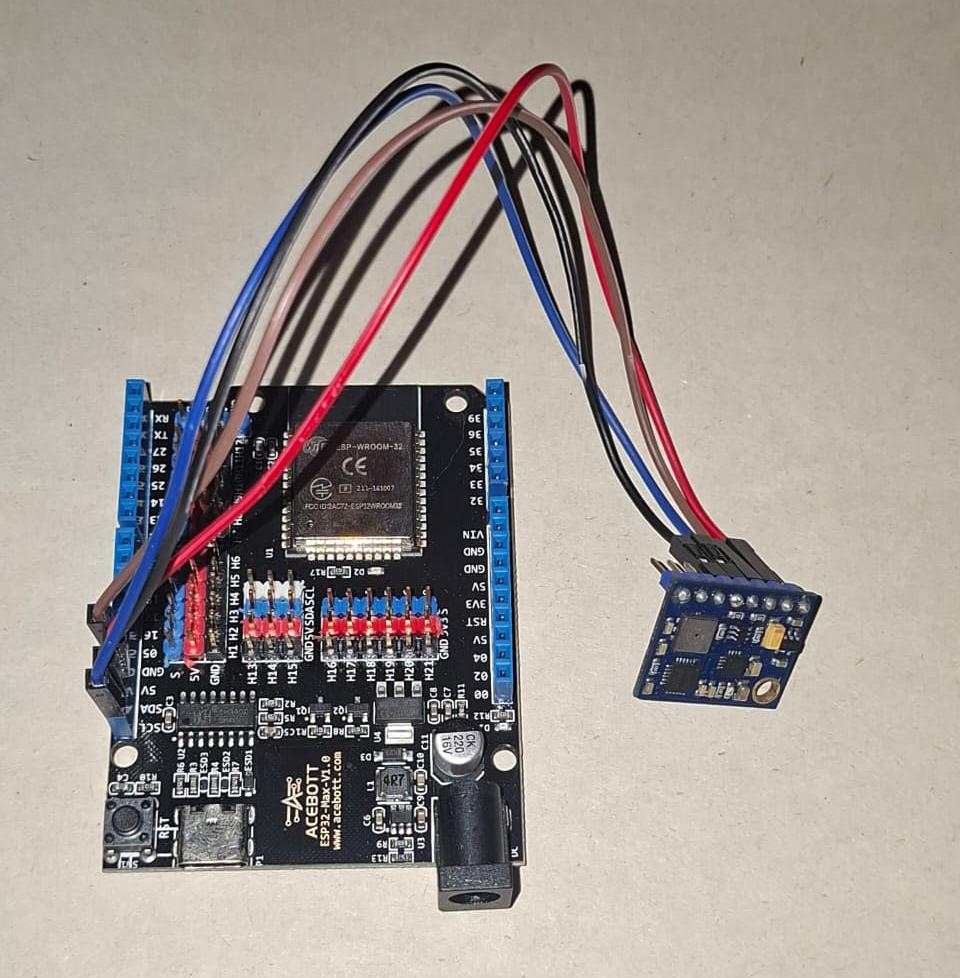
\includegraphics[width=0.4\textwidth]{figures/montaje.jpeg}
    \captionsetup{font=small, labelfont=bf}
    \caption{Montaje del sistema: ESP32 conectado al acelerómetro MPU6050.}
    \label{fig:montaje}
\end{figure}

\subsection{Clasificación en tiempo real}

La Figura~\ref{fig:serial} muestra una comparación del monitor serial del IDE de Arduino para los tres estados de movimiento. En cada caso, el modelo predijo correctamente la clase correspondiente: \texttt{0} para reposo, \texttt{1} para movimiento a la izquierda y \texttt{2} para movimiento a la derecha.

\begin{figure}[H]
    \centering
    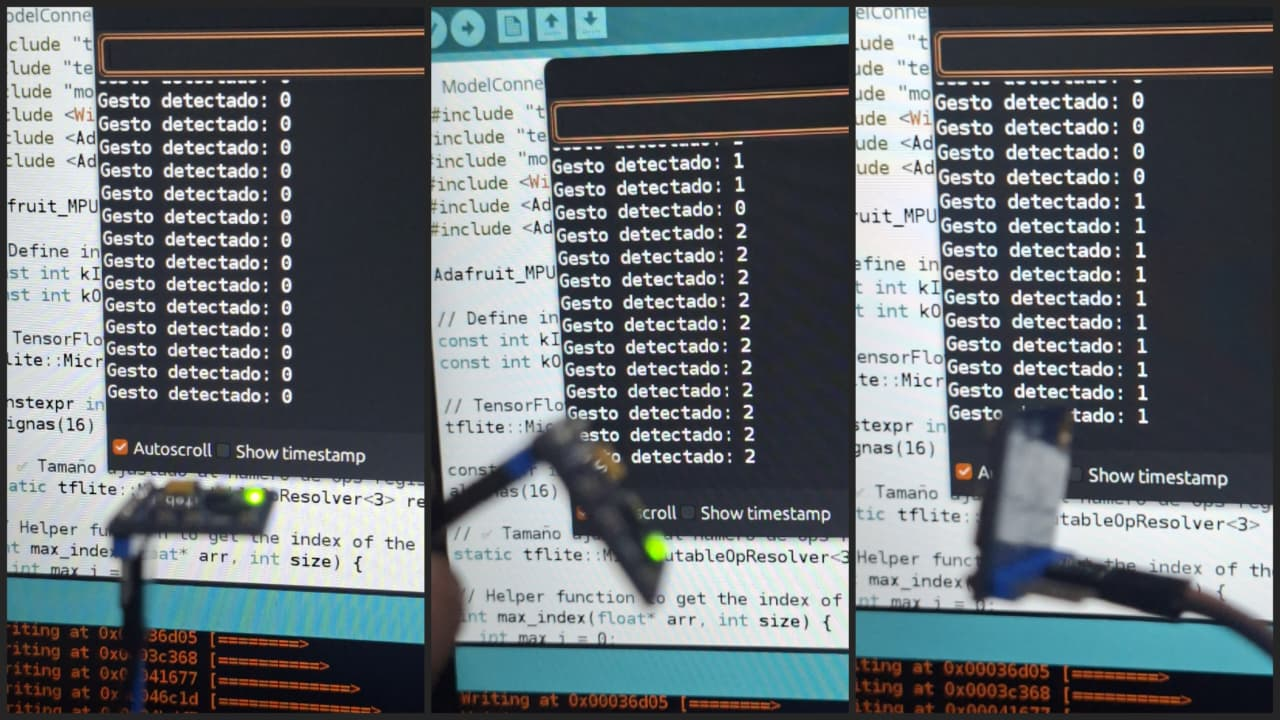
\includegraphics[width=0.4\textwidth]{figures/clasificacion-0-1-2.jpeg}
    \captionsetup{font=small, labelfont=bf}
    \caption{Monitor serial del ESP32 mostrando la clasificación correcta de los tres gestos (0 = reposo, 1 = izquierda, 2 = derecha).}
    \label{fig:serial}
\end{figure}

Los resultados muestran que el modelo logra identificar de manera consistente el tipo de movimiento, las probabilidades de salida de la red presentaron valores cercanos a 1.0 para la clase correcta en la mayoría de los casos, lo que indica una alta confianza en la predicción.

\subsection{Envío de datos a Firebase}

La Figura~\ref{fig:firebase} ilustra la interfaz de Firebase Realtime Database con los datos enviados por el ESP32, cada registro contiene el resultado de la clasificación y un identificador temporal, lo que permite monitorear el comportamiento del sistema de forma remota desde cualquier dispositivo con acceso a internet, además de un identificador único para cada registro.

\begin{figure}[H]
    \centering
    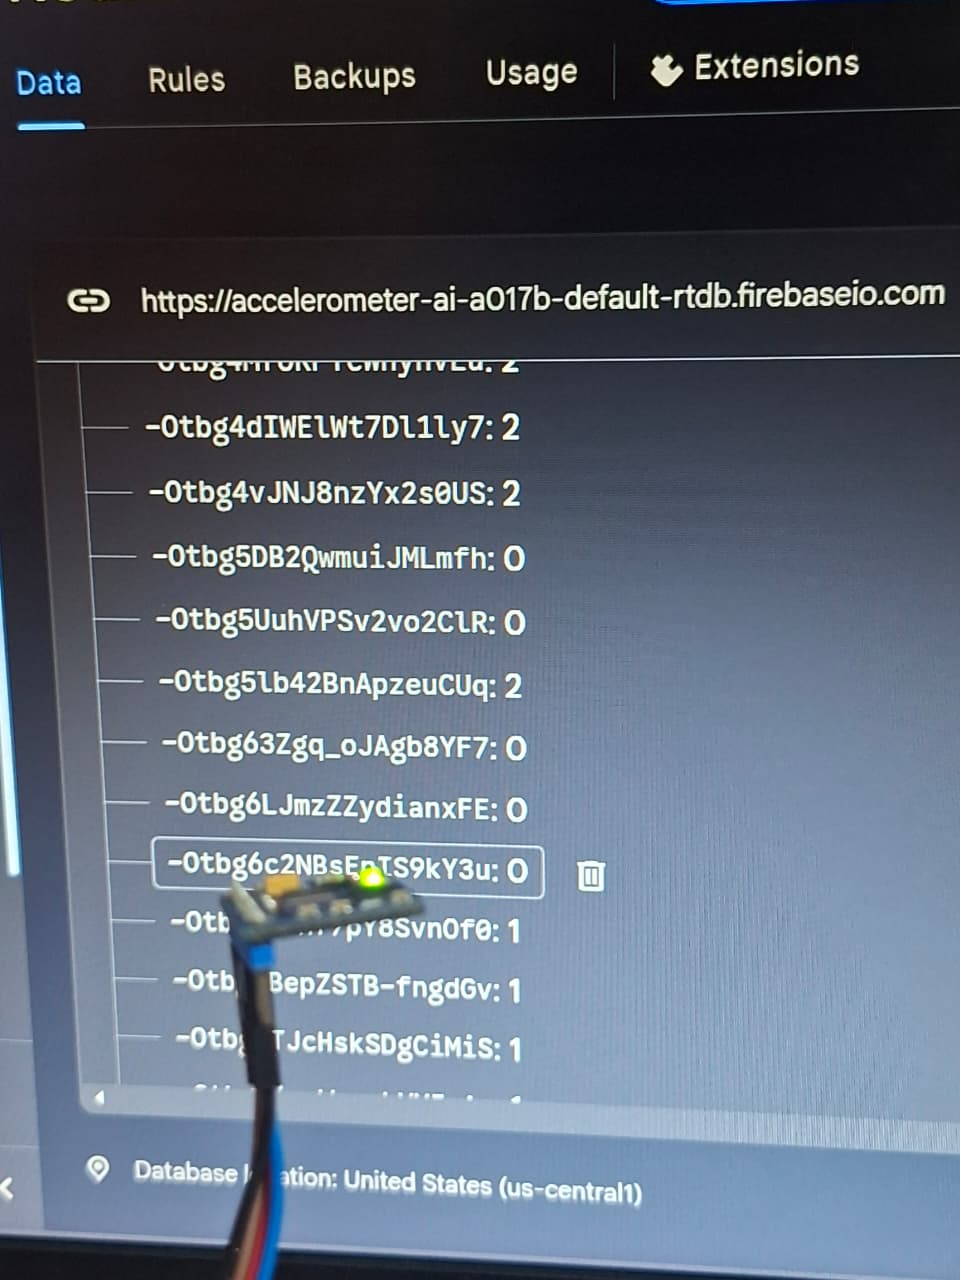
\includegraphics[width=0.2\textwidth]{figures/firebase.jpeg}
    \captionsetup{font=small, labelfont=bf}
    \caption{Comparación entre el gesto realizado físicamente y el registro correspondiente en la base de datos de Firebase.}
    \label{fig:firebase}
\end{figure}

En general, el sistema funcionó de acuerdo a lo esperado: el modelo de inteligencia artificial ejecutado en el ESP32 clasificó correctamente los movimientos y los datos fueron enviados y almacenados en la nube sin inconvenientes, si hubo desviaciones en algunos casos atribuibles a variaciones en la forma en que los gestos fueron realizados.

% ===================== 5. CONCLUSIONES =====================
\section{Conclusiones}

En esta práctica se implementó con éxito un sistema de clasificación de movimiento basado en TinyML, combinando el acelerómetro MPU6050, el microcontrolador ESP32 y un modelo de red neuronal densa ejecutado en formato TensorFlow Lite, el sistema demostró ser capaz de distinguir tres estados de movimiento en tiempo real con un alto grado de fiabilidad, y enviar los resultados a una base de datos en la nube, desde el punto de vista de la física experimental, este tipo de sistemas tiene aplicaciones directas en varias áreas como por ejemplo, en el estudio del movimiento de péndulos, osciladores o sistemas vibratorios, donde el acelerómetro puede reemplazar sensores más costosos y el modelo de IA puede identificar automáticamente regímenes de movimiento (libre, amortiguado, forzado) además de ser útil en sistemas de movimiento por levitación magnética, donde el acelerómetro puede comunicar información sobre el estado de movimiento a los electroimanes para corregir intensidades y configurar el movimiento. También resulta aplicable en experimentos de colisiones, donde la clasificación puede distinguir entre impactos elásticos e inelásticos a partir de los perfiles de aceleración, también en prácticas de mecánica de fluidos o de sismología a escala reducida, el sensor podría detectar patrones de vibración y clasificarlos de manera autónoma (proyecto actualmente en desarrollo en el laboratorio de instrumentación científica de la Universidad de Antioquia~\cite{pinpacho2025}).

Más allá del laboratorio, el paradigma TinyML tiene potencial en el desarrollo de instrumentación científica de bajo costo para regiones con recursos limitados, en sistemas de monitoreo remoto de estructuras o en dispositivos de asistencia que interpreten el movimiento corporal para aplicaciones médicas, la combinación de un sensor económico como el MPU6050 con un microcontrolador Wi-Fi como el ESP32 y una plataforma en la nube gratuita como Firebase hace que el sistema desarrollado sea replicable y escalable a problemas de mayor complejidad, además de una facilidad de acceso a los datos mediante Firebase, teniendo la capacidad de generar alertas en sistemas o comunidades enteras.

Como trabajo futuro, sería interesante aumentar el número de clases, hacer movimientos más complejos, incorporar los datos del giroscopio y explorar arquitecturas recurrentes (LSTM) para capturar la dinámica temporal de las señales de aceleración.

% ===================== REFERENCIAS =====================
\bibliographystyle{IEEEtran}
\bibliography{references}

\end{document}